\documentclass[dvipdfmx]{beamer}
\usepackage{setspace}
\usepackage{url}

\AtBeginDvi{\special{pdf:tounicode EUC-UCS2}}

\usetheme{Warsaw}
\setbeamertemplate{footline}[frame number]\renewcommand{\kanjifamilydefault}{\gtdefault}
\renewcommand{\kanjifamilydefault}{\gtdefault}

\title{GitとGitHubの小話}
\author{照井 章}
\institute{筑波大学 数理物質系}
\date{2019年6月18日}

\begin{document}
    
\begin{frame}
    \frametitle{}
    \titlepage
\end{frame}

\begin{frame}
    \frametitle{この話の内容}
    \large
    \setstretch{1.5}
    \begin{itemize}
        \item Git, GitHub とは何か?
        \item Git, GitHub の生い立ちなど
    \end{itemize}
\end{frame}

\begin{frame}
    \frametitle{Gitとは?}

    \begin{block}{バージョン管理システム (Version Management System)}
        \begin{itemize}
            \item コンピュータで編集されるファイルの変更履歴を管理するためのシステム
            \item 特にソフトウェア開発においてソースコードの管理に用いられることが多い
        \end{itemize}
    \end{block}

    \begin{flushright}
        出典: Wikipedia「バージョン管理システム」\cite{vcs}
    \end{flushright}
\end{frame}

\begin{frame}
    \frametitle{バージョン管理って?}
    複数人でソフトウェアを開発する際のソースコードの共有をどうするか?

    \begin{itemize}
        \item<1-> 2人の場合: ファイルをやりとりしあう(交換日記風)
        \item<2-> 3人: 3人の間でファイルが行ったり来たり
        \item<3-> もっと人数が増えると... どうする?
        \begin{itemize}
            \item<4-> 共通のファイルにみんなで書き込む
            \item<5-> 同じ箇所を2人が別々に書き換えたら?
            \item<6-> どの版が一番新しい?
            \item<7-> バグはどこで入った?
            \item<8-> etc.
        \end{itemize}
    \end{itemize}{}

    \only<9->{
        \begin{block}{}
            \begin{center}
                バージョン管理システムが解決する
            \end{center}
        \end{block}    
    }
\end{frame}

\begin{frame}
    \frametitle{これまでに登場したバージョン管理システム}
    \large
    \begin{itemize}
        \item SCCS
        \item RCS
        \item CVS
        \item Subversion
        \item Mercurial
        \item ...
    \end{itemize}
\end{frame}

\begin{frame}
    \frametitle{Gitの生みの親}
    \large
    Linus Tovalds (1969--)(写真は2014年)

    Linuxオペレーティングシステムの生みの親でもある

    \begin{center}
        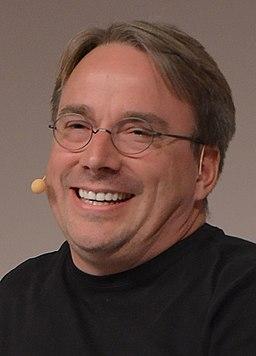
\includegraphics[scale=0.4]{256px-LinuxCon_Europe_Linus_Torvalds_03_(cropped).jpg}
        \\
        \small
        (出典: Wikimedia Commons, CC BY-SA 4.0)
    \end{center}
\end{frame}

\begin{frame}
    \frametitle{Gitが生まれたきっかけ \cite{git}}
    \large
    \begin{itemize}
        \item<1-> Linuxの開発には BitKeeper という商用のバージョン管理システムを使っていた
        \item<2-> BitKeeper は本来は有償だったが、Linuxの開発には無償で提供されていた
        \item<3-> しかし、2005年にあるLinux開発者とBitKeeperの開発元との間でトラブルが発生
        \item<4-> BitKeeperの開発元はBitKeeperの無償提供の終了を宣言
        \item<5-> Linus「それなら自分でバージョン管理システムを作る!」と宣言
        \item<6-> Gitが誕生 \cite{git-linux}
        \item<7-> 現在ではたくさんのソフトウェアの開発保守に使われている
    \end{itemize}
\end{frame}

\begin{frame}
    \frametitle{GitHub}
    \large
    \setstretch{1.5}
    \begin{itemize}
        \item ソースコードホスティングサービス
        \item Gitを使って管理を行う
        \item 2008年設立
        \item 2018年にMicrosoftに買収される
        \item 無料プランと有料プラン
        \begin{itemize}
            \item 有料プラン: 主に企業向け
            \item 無料プラン: 個人やオープンソースプロジェクト向け
            \item 2019年から、無料プランでもプライベートでリポジトリを無制限に作れるようになった(共同編集者は3人まで)
            \item 学生向けの優遇措置もある
        \end{itemize}
    \end{itemize}
\end{frame}

\begin{frame}
    \frametitle{GitHubの特徴}
    \large
    \setstretch{1.5}
    \begin{itemize}
        \item Gitのリポジトリホスティング
        \item forkとpull request
        \item ソースコードのレビュー
        \item 海外では大学のソフトウェア開発を伴う多くの授業でGitHubが使われている
    \end{itemize}
\end{frame}

\begin{frame}
    \frametitle{参考文献}
    \begin{thebibliography}{99}
        \bibitem{git} IDG Japan. BitKeeper紛争を受け、トーバルズ氏が新プロジェクト. ITMedia エンタープライズニュース, 2005年4月20日. \url{https://www.itmedia.co.jp/enterprise/articles/0504/20/news075.html} (参照 2019-06-17).
        \bibitem{git-linux} Linux.com, 江添亮(訳).gitの10周年を記念したLinus Torvalsへのインタビューの翻訳. 2015. \url{https://ezoeryou.github.io/blog/article/2015-04-08-linus-git-interview.html} (参照 2019-06-17).
        \bibitem{vcs} Wikipedia. バージョン管理システム. https://ja.wikipedia.org/wiki/バージョン管理システム (参照 2019-06-17).
    \end{thebibliography}    
\end{frame}

\end{document}